
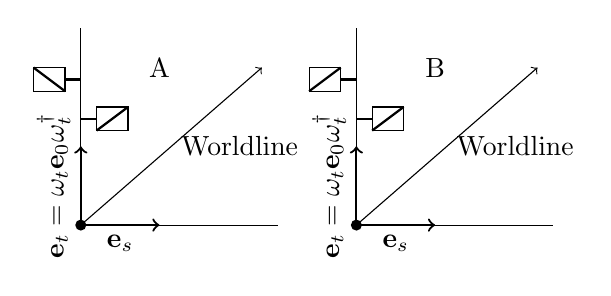
\begin{tikzpicture}
 % Define key coordinates A
 \coordinate (OriginA) at (0,0);
 \coordinate (TopYA) at (0,2.5);
 \coordinate (RighXA) at (2.5,0);
 \coordinate (StartWLA) at (0,0);
 \coordinate (EndWLA) at (2.3,2);

 % Flag 1 tips (Detached by 0.2, width 0.4)
 \coordinate (Flag1BottomLeft) at (0.2,1.2);
 \coordinate (Flag1BottomRight) at (0.6,1.2);
 \coordinate (Flag1TopLeft) at (0.2,1.5);
 \coordinate (Flag1TopRight) at (0.6,1.5);
 \coordinate (Arm1Pole) at (0,1.35);
 \coordinate (Arm1Flag) at (0.2,1.35);

 % Flag 2 tips
 \coordinate (Flag2BottomLeft) at (-0.2,1.7);
 \coordinate (Flag2BottomRight) at (-0.6,1.7);
 \coordinate (Flag2TopLeft) at (-0.2,2.0);
 \coordinate (Flag2TopRight) at (-0.6,2.0);
 \coordinate (Arm2Pole) at (0,1.85);
 \coordinate (Arm2Flag) at (-0.2,1.85);

 % Define key coordinates B
 \coordinate (OriginB) at (3.5,0);
 \coordinate (TopYB) at (3.5,2.5);
 \coordinate (RighXB) at (6.0,0);
 \coordinate (StartWLB) at (3.5,0);
 \coordinate (EndWLB) at (5.8,2);

 % Flag 3 tips
 \coordinate (Flag3BottomLeft) at (3.7,1.2);
 \coordinate (Flag3BottomRight) at (4.1,1.2);
 \coordinate (Flag3TopLeft) at (3.7,1.5);
 \coordinate (Flag3TopRight) at (4.1,1.5);
 \coordinate (Arm3Pole) at (3.5,1.35);
 \coordinate (Arm3Flag) at (3.7,1.35);

% Flag 4 tips
 \coordinate (Flag4BottomLeft) at (3.3,1.7);
 \coordinate (Flag4BottomRight) at (2.9,1.7);
 \coordinate (Flag4TopLeft) at (3.3,2.0);
 \coordinate (Flag4TopRight) at (2.9,2.0);
 \coordinate (Arm4Pole) at (3.5,1.85);
 \coordinate (Arm4Flag) at (3.3,1.85);
 
 % Draw the coordinate system A
 \fill (OriginA) circle (2pt) node[below left] {};
 \draw (OriginA) -- (RighXA);
 \draw (OriginA) -- (TopYA);
 \draw[thick, ->] (OriginA) -- ++(1,0) node[midway, below] {$\mathbf{e}_s$};
 \draw[thick, ->] (OriginA) -- ++(0,1) node[midway, left, rotate=90, anchor=south] {$\mathbf{e}_{t}=\boldsymbol{\omega}_{t}\mathbf{e}_{0}\boldsymbol{\omega}_{t}^{\dagger}$};
 
 % Draw Arm and Flag 1 (Scalar Base)
 \draw[thick] (Arm1Pole) -- (Arm1Flag);
 \draw (Flag1BottomRight) -- (Flag1BottomLeft) -- (Flag1TopLeft) -- (Flag1TopRight) -- cycle;
 \draw[thick] (Flag1BottomLeft) -- (Flag1TopRight);
 
 % Draw Arm and Flag 2 (Scalar Evolved - No Rotation)
 \draw[thick] (Arm2Pole) -- (Arm2Flag);
 \draw (Flag2BottomRight) -- (Flag2BottomLeft) -- (Flag2TopLeft) -- (Flag2TopRight) -- cycle;
 \draw[thick] (Flag2BottomLeft) -- (Flag2TopRight);
 
 % Draw worldline A
 \draw [->] (StartWLA) -- (EndWLA) node[midway, right] {Worldline};
 % Add an identification tag to diagram A
 \node at (1,2) {A};

 % Draw the coordinate system B
 \fill (OriginB) circle (2pt) node[below left] {};
 \draw (OriginB) -- (RighXB);
 \draw (OriginB) -- (TopYB);
 \draw[thick, ->] (OriginB) -- ++(1,0) node[midway, below] {$\mathbf{e}_s$};
 \draw[thick, ->] (OriginB) -- ++(0,1) node[midway, left, rotate=90, anchor=south] {$\mathbf{e}_{t}=\boldsymbol{\omega}_{t}\mathbf{e}_{0}\boldsymbol{\omega}_{t}^{\dagger}$};
 
 % Draw Arm and Flag 3 (Spinor Base)
 \draw[thick] (Arm3Pole) -- (Arm3Flag);
 \draw (Flag3BottomRight) -- (Flag3BottomLeft) -- (Flag3TopLeft) -- (Flag3TopRight) -- cycle;
 \draw[thick] (Flag3BottomLeft) -- (Flag3TopRight);
 
 % Draw Arm and Flag 4 (Spinor Twisted - 360 deg rotation)
 \draw[thick] (Arm4Pole) -- (Arm4Flag);
 \draw (Flag4BottomRight) -- (Flag4BottomLeft) -- (Flag4TopLeft) -- (Flag4TopRight) -- cycle;
 \draw[thick] (Flag4BottomRight) -- (Flag4TopLeft);


 % Draw worldline B
 \draw [->] (StartWLB) -- (EndWLB) node[midway, right] {Worldline};
 % Add an identification tag to diagram B
 \node at (4.5,2) {B};

\end{tikzpicture}
